\documentclass[../main.tex]{subfiles}
\begin{document}
\section{集合}
集合是近代数学的基本语言。用集合论重述人的直观经验,是近世数学和基于其构建的理论物理的普遍特点。连续介质力学中的大量概念都是依赖集合和映射来引入的。如果不熟悉集合和映射的语言和符号,就很难读懂后面的内容。

一般资料中常见的对集合的定义方式如下:

\begin{definition}\label{def:II.1.1}
    \emph{集合(set)}是具有某种特性的事物的整体。构成集合的事物或对象称为\emph{元素(element)}。集合还必须满足:
    \begin{itemize}
        \item 无序性:一个集合中,每个元素的地位是相同的,元素之间是无序的
        \item 互异性:一个集合中,任何两个元素都不相同,即每个元素只出现一次
        \item 确定性:给定一个集合及一个事物,该事物要么属于要么不属于该集合,不允许模棱两可。
    \end{itemize}
\end{definition}

定义\ref{def:II.1.1}的“确定性”,其实是逻辑学的排中律。具体地,若$A$是集合,$x$是$A$的一个元素,则记$x\in A$;若$y$不是$A$的元素,则记为$y\notin A$。记号“$x\in A$”规定了“$A$是集合且$x$是$A$的元素”。

如果只要有$x\in A$就有$x\in B$,则称$A$是$B$的\emph{子集(subset)},或称$A$包含于$B$、$B$包含$A$,记为$A\subset B$。显然,任一集合都是它自己的子集。

如果$A\subset B$且$B\subset A$,则集合$A$\emph{就是(is identical to)}B,记为$A=B$\footnote{此处等号“$=$”的意义应理解为:等号两边的字母是同一集合的不同代号。若写$A=B$,那么$A$\emph{就是}$B$。相应地,不等号“$\neq$”两边的字母是不同集合的代号。若写$A\neq B$,那么$A$\emph{不是}$B$。}。如果集合$A$与$B$的元素都相同,则$A$与$B$就是同一个集合。一个集合由其所有元素\emph{唯一}确定。这是集合论的\emph{外延公理(axiom of extension)}。

如果$A\subset B$且$A\neq B$,则称$A$是$B$的\emph{真子集(proper subset)},或称$A$真包含于$B$、$B$真包含$A$,记作$A\subsetneqq B$。

没有元素的集合称为\emph{空集(empty set)},记作$\emptyset$。空集是唯一的。简要证明:若$\emptyset_1$和$\emptyset_2$都是空集且$\emptyset_1\neq\emptyset_2$,则由空集的上述定义,要么存在$x\in\emptyset_1$且$x\notin\emptyset_2$,要么存在$y\in\emptyset_2$且$y\notin\emptyset_1$;无论哪种情况与$\emptyset_1$和$\emptyset_2$是空集相矛盾。因此要么$\emptyset_1$和$\emptyset_2$有一个不是空集,要么它们是同一个集合,即“空集是唯一的”。

给定一个集合$A$,我们可以根据$A$的元素所需要满足的附加要求,构建出$A$的子集。例如,设$A$是所有偶数的集合,附加的要求是“比1大、比9小”,我们就从$A$中找出了2、4、6、8这四个元素组成的集合$B$。一般地,我们将此记作:
\[
    \left\{x\in A|\text{$x$需要满足的条件}\right\}
\]
注意,预先给定一个基本集合$A$这一步原则上是不可省略的;“|”后的语句形式是对$A$的元素$x$的规定,而不能是其他意义。这是集合论的\emph{分类公理(axiom of specification)}。

给定两个集合$A$和$B$,总存在唯一一个这样的集合$V$:只要$x\in V$,就有$x\in A$且$x\in B$;反之,若$x\in A$且$x\in B$,则有$x\in V$。这样的集合$V$的存在性来自分类公理;$V$可表示成:
\[
    V=\left\{x\in A|x\in B\right\}
\]
$V$的唯一性简证如下:若另有一$V^\prime=\left\{x\in A|x\in B\right\}$且$V^\prime\neq V$,则由外延公理必存在$x\in V^\prime$且$x\notin V$。若$x\in V^\prime$,则$x\in A$且$x\in B$;若$x\notin V$,则$x\notin A$或$x\notin B$,这两个推论相互矛盾\footnote{由集合定义\ref{def:II.1.1}中的“确定性”。}。因此$V^\prime=V$或$V^\prime$不存在,即$V$是唯一的。我们把这样的集合$V$称作集合$A$与$B$的\emph{交集(interset)},记作$V=A\cap B$。

我们经常还要讨论“集合的集合”,从而有“元素的元素”。

设$\mathcal{C}$是集合的集合,且$\mathcal{C}\neq\emptyset$。设$A\in\mathcal{C}$,则由分类公理存在以下集合
\[
    V=\left\{x\in A|x\in X\Leftrightarrow X\in\mathcal{C}\right\}
\]
其中$\Leftrightarrow$是\emph{当且仅当(if and only if,iff)}的意思。这一集合$V$的唯一性可类似上一段那样得证,此略\footnote{下文构建的集合的唯一性,不作说明时,都由外延公理保证。}。我们称$V$是$\mathcal{C}$的元素的交集,记作
\[
    V=\bigcap_{X\in\mathcal{C}}X
\]

集合的交集有如下性质:
\begin{enumerate}
    \item $A\cap\emptyset=\emptyset$
    \item $A\cap B=B\cap A$(交换律)
    \item $A\cap\left(B\cap C\right)=\left(A\cap B\right)\cap C$(结合律)
    \item $A\cap A=A$(幂等)
    \item $A\subset B\Leftrightarrow A\cap B=A$
\end{enumerate}

如果集合$A$和$B$的交集是空集,即$A\cap B=\emptyset$,则称$A$与$B$是\emph{不相交的(disjoint)}。比如,我们有时会说,某集合的集合$\mathcal{C}$中的元素\emph{两两不相交(pair-wise disjoint)}。

分类公理只允许我们“收窄”一个给定的集合。以下规定的原则将允许我们从已有集合构建出“更大的”集合。

我们可以把任意两个集合$a$、$b$组成一对,变成一个新的集合,记作$\left\{a,b\right\}$,并\emph{规定}这样的集合可以存在。这是集合论的\emph{配对公理(axiom of paring)}。于是有$a\in \left\{a,b\right\}$和$b\in \left\{a,b\right\}$。特别地,一个集合$a$可与其自身“成对”,得到“$\left\{a,a\right\}$”,但由于集合的元素要满足互异性,故实际所得到的集合应是$\left\{a\right\}$。这种只有一个元素的集合,称为\emph{单元素集(singleton)}。注意理解以下事实:$\emptyset\in\left\{\emptyset\right\}$,$\left\{\emptyset\right\}\neq\emptyset$。

我们可以让若干个集合形成并集。具体地,我们\emph{规定}对任意集合的集合$\mathcal{C}$,总存在一个集合$U$,它含有$\mathcal{C}$的至少一个元素的所有元素\footnote{$\mathcal{C}$的元素是集合。}。这样规定存在的集合$U$,还可能包含不属于$\mathcal{C}$中任一集合的元素。但是我们总是可以再利用分类公理,把$U$收窄为恰好只包含$\mathcal{C}$中的所有元素的所有元素。具体地,给定一个集合的集合$\mathcal{C}$,由并集公理必存在上述的$U$,利用分类公理构建以下集合\footnote{符号$\exists$表示“存在一个”或“给定一个”的意思。符号$\wedge$表示“且”的意思。}
\begin{equation*}\label{eq:set_union}
    \left\{x\in U|\exists X\left(X\in\mathcal{C}\wedge x\in X\right)\right\}
\end{equation*}
使得对每一$x\in U$,当且仅当$x$属于$\mathcal{C}$的某个元素$X$,$x$属于上列集合。因此上列集合包括且仅包括$\mathcal{C}$中的所有元素的所有元素。我们称上列集合为$\mathcal{C}$的所有元素的\emph{并集(union)},记作
\[
    \bigcup_{X\in\mathcal{C}}X
\]
这是集合论的\emph{并集公理(axiom of unions)}。特别地,若$\mathcal{C}=\emptyset$,则$\bigcup_{X\in\mathcal{C}}X=\emptyset$,简单证明:由并集的定义,若存在$a\in\bigcup_{X\in\mathcal{C}}X$,则至少存在一个$X\in\mathcal{C}=\emptyset$满足$x\in X$,但是显然不存在属于空集的元素$X$,因此不存在所述的$a$,即$\bigcup_{X\in\mathcal{C}}X$是空集。

如果$\mathcal{C}$是由两个集合$A$和$B$配对而成,即$\mathcal{C}=\left\{A,B\right\}$,则$\mathcal{C}$的元素的并集常以中缀的记法写成:
\[
    \bigcup_{X\in\left\{A,B\right\}}X= A\cup B
\]

集合的并集有如下性质:

\begin{enumerate}
    \item $A\cup \emptyset=A$
    \item $A\cup B=B\cup A$(交换律)
    \item $A\cup\left(B\cup C\right)=\left(A\cup B\right)\cup C$(结合律)
    \item $A\cup A=A$(幂等)
    \item $A\subset B\Leftrightarrow A\cup B=B$
\end{enumerate}

我们利用并集操作把若干个单元素集结合成一个含有限个元素的集合。例如,
\[
    \left\{a,b,c\right\}=\left\{a\right\}\cup\left(\left\{b\right\}\cup\left\{c\right\}\right)=\left(\left\{a\right\}\cup\left\{b\right\}\right)\cup\left\{c\right\}=\bigcup_{X\in\left\{\left\{a\right\},\left\{b\right\},\left\{c\right\}\right\}}X
\]
依此类推,任意有限个元素的集合都可由此方法构建\footnote{至此,我们可以回过头来重新理解集合的定义\ref{def:II.1.1}中的“无序性”、“互异性”和“确定性”。头两个规定,其实是外延公理的推论。例如,若集合$A=\left\{a,b,c\right\}$,$B=\left\{c,b,a\right\}$,则由外延公理$A=B$(无序性)。若集合$A=\left\{a,a\right\}$,$B=\left\{a\right\}$,则由外延公理$A=B$(互异性)。最后,定义\ref{def:II.1.1}中的“确定性”,只是逻辑上排中律的要求。}。

给定集合$A$和$B$,集合$C=\left\{x\in A|x\notin B\right\}$称$B$在$A$中的\emph{相对补集(relative complement of $B$ in $A$)},记为$C=A\setminus B$。注意,此处$B$不必包含于$A$。

我们常在给定一个全集$E$之下讨论其子集在$E$中的相对补集。如果默认这一前提,则可简称任一$E$的子集$A\subset E$在$E$中的相对补集为$A$的补集,记为$A^\complement\equiv E\setminus A$\footnote{有时,我们使用恒等号“$\equiv$”来表示新引入的符号或者记法代表什么表达式。}。

给定全集$E$下集合的补集有如下性质:
\begin{enumerate}
    \item $\left(A^\complement\right)^\complement=A$
    \item $\emptyset^\complement=E$
    \item $E^\complement=\emptyset$
    \item $A\cap A^\complement=\emptyset$
    \item $A\cup A^\complement=E$
    \item $A\subset B\Leftrightarrow B^\complement\subset A^\complement$
\end{enumerate}

关于集合的并集、交集,以及给定全集下的补集还有一条重要定律——\emph{德摩根定律(De Morgan's Laws)}:对任意集合$A$、$B$,有
\begin{align*}
    \left(A\cup B\right)^\complement & =A^\complement\cap B^\complement \\
    \left(A\cap B\right)^\complement & =A^\complement\cup B^\complement
\end{align*}

给定一个集合$A$,我们\emph{规定}存在一个集合,暂记作$\mathcal{P}^\prime\left(A\right)$,它包含所有$A$的子集。这是集合论的\emph{幂集公理(axiom of powers)}。我们于是可遵守分类公理给出恰好包括$A$的所有子集(包括空集和集合$A$本身),而不包括其他元素的集合:
\[
    \mathcal{P}\left(A\right)=\left\{X\in\mathcal{P}^\prime\left(A\right)|X\subset A\right\}
\]
我们称$\mathcal{P}\left(A\right)$为集合$A$的\emph{幂集(power set)}。

为什么把这样的集合称为“幂集”呢?若$A=\emptyset$,则$\mathcal{P}\left(A\right)=\left\{\emptyset\right\}$,有$1=2^0$个元素;若$A=\left\{a\right\}$,则$\mathcal{P}\left(A\right)=\left\{\emptyset,\left\{a\right\}\right\}$,有$2=2^1$个元素;若$A=\left\{a,b\right\}$,则$\mathcal{P}\left(A\right)=\left\{\emptyset,\left\{a\right\},\left\{b\right\},\left\{a,b\right\}\right\}$,有$4=2^2$个元素;……

注意到,若$X\in\mathcal{P}\left(E\right)$,则有$X^\complement\in\mathcal{P}\left(E\right)$。于是,默认以$E$为全集时,我们不必逐个讨论$E$的子集的补集。设$\mathcal{C}\subset\mathcal{P}\left(E\right)$,则$\mathcal{C}$中的元素的补集的集合为
\[
    \mathcal{D}=\left\{X\in\mathcal{P}\left(E\right)|X^\complement\in\mathcal{C}\right\}
\]
这时,德摩根定律有如下更一般的形式:
\begin{align*}
    \left(\bigcup_{X\in\mathcal{C}}X\right)^\complement=\bigcap_{X\in\mathcal{C}}X^\complement \\
    \left(\bigcap_{X\in\mathcal{C}}X\right)^\complement=\bigcup_{X\in\mathcal{C}}X^\complement
\end{align*}
其中我们引入了以下记法惯例:
\[
    \bigcap_{X\in\mathcal{C}}X^\complement\equiv\bigcap_{X\in\mathcal{D}}X, \bigcup_{X\in\mathcal{C}}X^\complement\equiv\bigcup_{X\in\mathcal{D}}X
\]

由集合的定义\ref{def:II.1.1}所要求的无序性,给定两个集合$a$、$b$,它们的配对集合$\left\{a,b\right\}$是不表示顺序的。我们可以用$a$的单元素集$\left\{a\right\}$和$\left\{a,b\right\}$这两个集合,配对得到集合$\left\{\left\{a\right\},\left\{a,b\right\}\right\}\equiv\left(a,b\right)$,来表示\emph{有序对(ordered pair)}。在$\left(a,b\right)$的元素中,$\left\{a,b\right\}$表明我们讨论哪两个元素的有序对,而$\left\{a\right\}$表明哪一个元素放在前面。所以,$\left(a,b\right)\neq\left(b,a\right)$。

给定两个集合$A$、$B$,是否可以给出所有$a\in A$且$b\in B$的有序对$\left(a,b\right)$的集合?我们留意到,对任意$a\in A$和$b\in B$有$\left\{a\right\}\subset A$,$\left\{b\right\}\subset B$,$\left\{a,b\right\}\subset A\cup B$,$\left\{a\right\}\subset A\cup B$。可见,$\left\{a\right\}$和$\left\{a,b\right\}$都是集合$A\cup B$的子集,故$\left(a,b\right)\in\mathcal{P}\left(A\cup B\right)$,$\left(a,b\right)\subset\mathcal{P}\left(\mathcal{P}\left(A\cup B\right)\right)$。换言之,只要$a\in A$且$b\in B$,就有$\left(a,b\right)\subset\mathcal{P}\left(\mathcal{P}\left(A\cup B\right)\right)$。于是我们可以遵循分类公理,把所有$a\in A$且$b\in B$的有序对$\left(a,b\right)$的集合规定出来,且其唯一性由外延公理保证\footnote{
    用分类公理、并集公理、配对公理和幂集构建集合$A$与$B$的笛卡尔集的过程,用自然语言描述将十分繁琐。以下是采用\emph{合式公式(well-formed formula)}表达的结果,仅供熟悉此知识的读者参考。
    \[A\times B=\left\{X\in\mathcal{P}\left(\mathcal{P}\left(A\cup B\right)\right)|\varphi\left(X\right)\right\}
    \]
    其中,$\varphi\left(X\right)$表示关于$X$的语句,
    \[
        \varphi\left(X\right)=\exists U\exists V\exists W \exists Y\left(U\in A \wedge V\in B\wedge \phi\left(W,U,U\right)\wedge\phi\left(Y,U,V\right)\wedge\phi\left(X,W,Y\right)\right)
    \]
    而关于$X$、$U$和$V$的语句
    \[
        \phi\left(X,U,V\right)=\forall Z\left(Z\in X\leftrightarrow\left(\left(X=U\right)\vee\left(X=V\right)\right)\right)
    \]
    其中,记号$\forall a\left(\text{关于$a$的语句}\right)$表示“对每一/任一满足关于$a$的语句规定的$a$”。注意到,语句$\phi\left(X,U,V\right)$表示的就是$X=\left\{U,V\right\}$这件事,故语句$\varphi\left(X\right)$就是让$X=\left\{\left\{U\right\},\left\{U,V\right\}\right\}$。
}。故我们可定义由集合$A$和$B$形成的所有满足$a\in A$且$b\in B$的有序对的集合为$A$与$B$的\emph{笛卡尔积(Cartesian product)},记为$A\times B$。

以下是与笛卡尔集有关的一些性质:
\begin{enumerate}
    \item $\left(A\cup B\right)\times X=\left(A\times X\right)\cup\left(B\times X\right)$
    \item $\left(A\cap B\right)\times \left(X\cap Y\right)=\left(A\times X\right)\cap\left(B\times Y\right)$
    \item $\left(A\setminus B\right)\times X=\left(A\times X\right)\setminus \left(B\times X\right)$
    \item $A=\emptyset\text{或}B=\emptyset\Leftrightarrow A\times B=\emptyset$
    \item $A\subset X\text{且}B\subset Y\Rightarrow A\times B\subset X\times Y$\footnote{符号$\Rightarrow$的意义:(语句1)$\Rightarrow$(语句2)表示“若(语句1 ),则(语句2)。”}
    \item $A\times B\subset X\times Y\text{且}A\times B\neq\emptyset\Rightarrow A\subset X\text{且}B\subset Y$
\end{enumerate}

不难留意到,笛卡尔积运算不满足交换律和结合律。

多于两个集合的笛卡尔集的严格定义,需要在介绍完映射的概念后才能给出。

%====================
\section{关系}
一个集合的元素可与另一个集合的元素形成对应关系。例如,设$A$是所有成年公民的集合,那么“婚姻”就是定义在$A$的任意两个不同元素之间的关系。每对夫妻都是一个有序对$\left(a,b\right)\in A\times A$。在实际社会生活中,我们是先用其他概念对婚姻关系进行定义(例如当地的《婚姻法》),再辨别任意两个公民之间是否具有婚姻关系的。但是在集合论中,我们没有超出集合论的其他概念以供我们独立地定义元素间的一种关系。我们只能视符合某关系的\emph{所有}有序对的集合为这一关系的定义。例如,我们不采用既有的《婚姻法》来定义何谓婚姻关系,而是把所有具有合法婚姻关系的公民对全部列出来组成一个集合,作为关于“何谓婚姻关系”的一种完整的界定。要辩认$a, b\in A$是否婚姻关系,就只看有序对$\left(a,b\right)$是否属于上述集合。这种定义关系的方法才是集合论可以普适地采用的。

正式地,若集合$R$的元素都是有序对,则集合$R$就是一个\emph{关系(relation)}。若有序对$\left(x,y\right)\in R$,则记为$xRy$。习惯上,一般的关系常用符号“$\sim$”表示,各种特殊的关系会用特定的符号表示。设$\sim$是一个关系,若$\left(x,y\right)\in \sim$,则$x\sim y$;若$\left(x,y\right)\notin\sim$,则记为$x\not\sim y$。关系的定义告诉我们:

\begin{figure}[htbp]
    \centering
    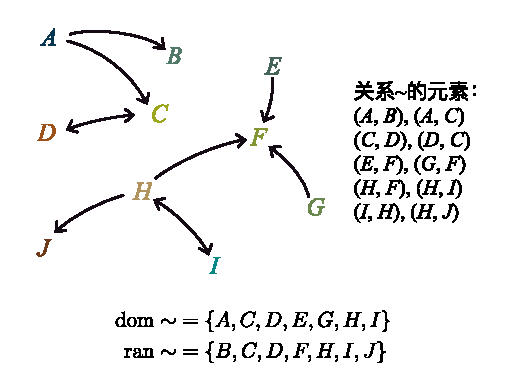
\includegraphics{../images/relation.pdf}
    \caption{图中展示了一个关系$\sim$。箭头表示一个有序对中两个元素的先后次序。}
    \label{fig:II.1.1}
\end{figure}

\begin{enumerate}
    \item 关系$\sim$是一个有序对的集合。图\ref{fig:II.1.1}的箭头表示法可协助我们把“有序对的集合”联系到“关系”一词的日常意义。
    \item 任一关系$\sim$总可以写成两个集合的笛卡尔积的子集。证明的方法:验证关系$\sim$至少可以是下列笛卡尔积
          \[
              \left(\bigcup_{X\in\bigcup_{X^\prime\in\sim}X^\prime}X\right) \times\left(\bigcup_{X\in\bigcup_{X^\prime\in\sim}X^\prime}X\right)
          \]
          的子集\footnote{提示:回顾有序对的定义$\left(a,b\right)\equiv\left\{\left\{a\right\},\left\{a,b\right\}\right\}$,把表达式
              \[
                  \bigcup_{X\in\bigcup_{X^\prime\in\sim}X^\prime}X
              \]
              所形成的集合写出来,可以发现它是关系$\sim$的所有有序对中的元素的集合。读者可以尝试以图\ref{fig:II.1.1}的例子写出图中关系的$\bigcup_{X\in\bigcup_{X^\prime\in\sim}X^\prime}X$;它就是$\left\{A,B,C,D,E,F,G,H,I,J\right\}$。}
    \item 关系的元素未必是同一个集合与其自身的笛卡尔集。两个不同集合$X$与$Y$之间也可以定义某关系$\sim\subset X\times Y$。只要$x\in X,y\in Y,\left(x,y\right)\in\sim$,则$x\sim y$。若$\sim\subset X\times X$,则称“$\sim$是集合$X$上的关系”;若$\sim\subset X\times Y$,则称“$\sim$是从集合$X$到集合$Y$的关系”。
\end{enumerate}

\begin{example}
    设$A=\left\{a,b\right\}, B=\left\{1,2\right\}$,则$A\times B=\left\{\left(a,1\right),\left(a,2\right),\left(b,1\right),\left(b,2\right)\right\}$。设关系$\sim=\left\{\left(a,1\right),\left(b,2\right)\right\}$。我们不难留意到,$\sim\subset A\times B$。按照关系$\sim$的定义,我们可以写$a\sim 1,a\not\sim 2$。

    留意到,$A\times B$本身就是一个关系。若$\sim=A\times B$,则$A$的任一元素与$B$的任一元素之间都有$\sim$关系,即$\forall a\in A\forall b\in B,a\sim b$。

    等于“$=$”关系是任一集合与其自身的笛卡积的子集。具体地,设$X$是一个非空集合,则$X\times X$中所有满足$x=y$的有序对$\left(x,y\right)$的集合就是等于关系。

    属于“$\in$”也是一个关系。具体地,它是$X\times\mathcal{P}\left(X\right)$满足$x\in A$的所有有序对$\left(x,A\right)$的集合。

    空集是有序对的集合(因为空集是集合,且空集不含有任何不是有序对的元素),因此空集也可以是一个关系。
\end{example}

接上列的第2条,给定一个关系$\sim$,记$U_\sim\equiv\bigcup_{X\in\bigcup_{X^\prime\in\sim}X^\prime}X$,遵循分类公理所构建的集合
\[
    \left\{a\in U_\sim|\exists b\left(b\in U_\sim\wedge a\sim b\right)\right\}
\]
为关系$\sim$的\emph{定义域(domain)},记作$\mathrm{dom}\sim$。集合
\[
    \left\{b\in U_\sim|\exists a\left(a\in U_\sim\wedge a\sim b\right)\right\}
\]
为关系$\sim$的\emph{值域(range)},记作$\mathrm{ran}\sim$。图\ref{fig:II.1.1}给出了所示关系的定义域和值域。不难留意到,对于任一集合上的等于关系,有$\left(\mathrm{dom}=\right)=\left(\mathrm{ran}=\right)$;对于任一集合上的属于关系,若$\left(\mathrm{dom}\in\right)=X$,则$\left(\mathrm{ran}\in\right)=\mathcal{P}\left(X\right)\setminus\left\{\emptyset\right\}$\footnote{因为$\emptyset\in\mathcal{P}\left(X\right)$,但没有元素能够属于$\emptyset$。}。

\begin{definition}[等价关系]\label{def:II.1.2}
    设$\sim$是集合$X$上的一个关系。若
    \begin{enumerate}
        \item 对任一$x\in X$都有$x\sim x$,则称关系$\sim$是\emph{自反的(reflextive)}。
        \item 对任意$x\in X$和$y\in X$,只要$x\sim y$就有$y\sim x$,则称关系$\sim$是\emph{对称的(symmetric)}。
        \item 对任意$x\in X$、$y\in X$和$z\in X$,只要$x\sim y\text{且}y\sim z$就有$x\sim z$,则称关系$\sim$是\emph{传递的(transitive)}
    \end{enumerate}
    若集合$X$上的一个关系$\sim$同时满足上述3个性质,则称$\sim$是$X$上的一个\emph{等价关系(equivalent relation)}。
\end{definition}

以图\ref{fig:II.1.1}为例,如果图\ref{fig:II.1.1}中的每个元素都有一个从自己回到自己的箭头,那么图中的关系就是自反的;如果图\ref{fig:II.1.1}中的所有箭头都是双向箭头,那么图中的关系就是对称的。读者可尝试把图\ref{fig:II.1.1}的关系修改成非自反、非对称,但传递的关系\footnote{注意这几条定义所要求的“对任意……”,只要有一个例外就可以失效。}。

\begin{example}
    设$X=\left\{a,b,c\right\}$。$X$上的等于关系是$X$上的等价关系。它是集合
    \[
        \left\{\left(a,a\right),\left(b,b\right),\left(c,c\right)\right\}
    \]
    这一集合共有3个元素。同时,$X\times X$也是$X$上的等价关系,它有$2^3=8$个元素。

    一般地,任一非空集合$X$上的等于关系是$X$上的(除空集外)“最小”的等价关系,$X\times X$是$X$上的最大等价关系。

    不等于$\neq$只满足对称性。

    任意集合的包含关系具有自反性和传递性,但集合的包含关系没有对任意集合均成立的对称性。事实上,在上一节关于外延公理的段落中已经介绍过,具有对称性的包含关系就是集合的等于关系。

    显然,“婚姻”不是“全体成年公民”集合上的等价关系。“婚姻”只满足对称性。
\end{example}

此时我们回过头讨论集合论最基本的关系——从属关系的自反性、对称性和传递性。从属关系的自反性是指,一个集合$A$属于它自己,$A\in A$。从属关系的对称性是指,$A\in B\Leftrightarrow B\in A$。从属关系的传递性是指,$A\in B \wedge B\in C\Rightarrow A\in C$。直觉上,这三种性质都不令人舒适,但它们未被直至目前的讨论所禁止。若想禁止上述性质,需要\emph{正则公理(axiom of regularity)}:给定任一非空集合$X$,则$X$中必含有一个元素$y\in x$满足$y\cup X=\emptyset$,用符号表述为$X\neq \emptyset\Rightarrow\exists y\left(y\in X\wedge y\cup X=\emptyset\right)$。正则公理同时禁止了三种性质(证明从略)。本讲义所使用的集合论遵循正则公理。

\begin{figure}[htbp]
    \centering
    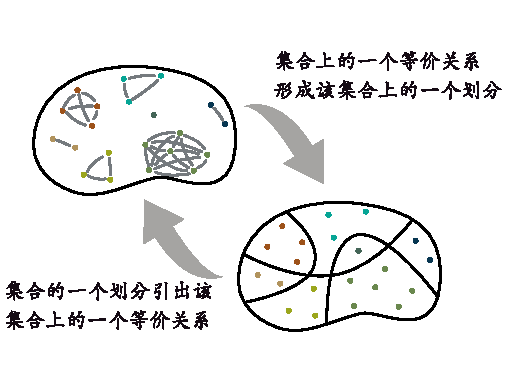
\includegraphics[width=0.5\textwidth]{../images/partition.pdf}
    \caption{集合的划分与集合上的等价关系}
    \label{fig:II.1.2}
\end{figure}

回到等价关系的讨论。如果集合$X$的非空子集的集合$\mathcal{C}$满足$\bigcup_{Y\in\mathcal{C}}Y=X$且$\mathcal{C}$的元素两两不相交,则称集合$\mathcal{C}$是$X$的一个\emph{划分(partition)}。换言之,如果$X$的若干个非空子集两两不相交,但它们的并集又恰好得到$X$,那么这些子集就好像对集合$X$进行“切蛋糕”所得到结果(如图\ref{fig:II.1.2}右下的情况)。

若集合$\mathcal{C}$是集合$X$的一个划分,我们可以由此定义一个关系$\sim\equiv X/\mathcal{C}$\footnote{该记法与刚刚介绍完的$X/\sim$无关,是符号“$/$”的滥用。},使得当且仅当$X$的元素$x,y$属于$\mathcal{C}$的同一个元素时,$x\sim y$。正式地,
\begin{equation}\label{eq:relation_induced_by_partition}
    X/\mathcal{C}=\left\{\left(x,y\right)\in X\times X|\exists A\left(A\in \mathcal{C}\wedge\left\{x,y\right\}\subset A\right)\right\}
\end{equation}
图\ref{fig:II.1.2}中,将右下所示的集合的划分中同属一个子集的元素两两连线,就能得到左上所示的关系。这一关系在给定划分$\mathcal{C}$下的唯一性由外延公理保证。

可以证明,这一关系是等价关系:
\begin{proof}
    验证关系$\sim\equiv X/\mathcal{C}$是等价关系,需一一验证其自反性、对称性和传递性。
    \begin{enumerate}
        \item 自反性:需证明对任意$x\in X$,有序对$\left(x,x\right)\in\sim$。这需要:
              \begin{enumerate}
                  \item $\left(x,x\right)\in X\times x$。由$x\in X$这显然满足。
                  \item $\exists A\in\mathcal{C},x\in A$。由并集的定义(式\eqref{eq:set_union}),$\mathcal{C}$作为一个集合的集合,对任一$x\in\bigcup_{A\in\mathcal{C}}A$必存在$A\in\mathcal{C}$满足$x\in A$。现在$\mathcal{C}$是集合$X$的一个划分,即$\bigcup_{A\in\mathcal{C}}A=X$,故对任一$x\in X$必存在$A\in\mathcal{C}$满足$x\in A$。自反性证毕。
              \end{enumerate}
        \item 对称性:需证明$\left(x,y\right)\in\sim\Leftrightarrow\left(y,x\right)\in\sim$,其中$x,y\in X,x\neq y$。显然,由于$x,y\in X$,$\left(x,y\right)\in X\times X$且$\left(Y,x\right)\in X\times X$。若$\left(x,y\right)\in\sim$,则由$\sim$的定义$\exists A\in\mathcal{C}\left\{x,y\right\}\subset A$,故自然有$\left(y,x\right)\in\sim$;反之亦然。对称性证毕。
        \item 传递性:需证明$\left(x,y\right)\in\sim\wedge\left(y,z\right)\in\sim\Rightarrow\left(x,z\right)\in\sim$,其中$x,y,z\in X,x\neq y,x\neq z,y\neq z$。显然,由于$x,z\in X$,$\left(x,z\right)\in X\times X$。由$\sim$的定义,$x\sim y\Rightarrow\exists A\in\mathcal{C},\left\{x,y\right\}\subset A$,$y\sim z\Rightarrow\exists A^\prime\mathcal{C},\left\{y,z\right\}\subset A^\prime$。由于$\mathcal{C}$是$X$的一个划分,由划分的定义,要么$A=A^\prime$,要么$A\cap A^\prime=\emptyset$,故$A=A^\prime$,即$\left\{x,y,z\right\}\subset A$。再由关系$\sim$的定义有$x\sim z$。传递性证毕。
    \end{enumerate}
\end{proof}
因此我们称式\eqref{eq:relation_induced_by_partition}定义的等价关系是\emph{由集合$X$的划分$\mathcal{C}$引出的等价关系(equivalent relation induced by the partition $\mathcal{C}$ of $X$)}。

上一段介绍的是图\ref{fig:II.1.2}右下到左上的定理,下面我们将介绍相当于图\ref{fig:II.1.2}中从左上到右下的定理。

设关系$\sim$是集合$X$上的一个等价关系,则集合$\left\llbracket x\right\rrbracket_\sim\equiv\left\{y|y\in X\wedge\left(\exists x\in X,y\sim x\right)\right\}$称$x$关于$\sim$的\emph{等价类(equivalent class)}\footnote{“类”与“集合”在概念上无实质区别。}。$X$的元素关于$\sim$的所有等价类的集合,记作$X/\sim$\footnote{注意与相对补集的符号相区别。},称为集合$X$在等价关系$\sim$下的\emph{商集(quotient set)}\footnote{正式地,
    \[
        X/\sim\equiv\left\{A\in\mathcal{P}\left(X\right)|\forall x\left(x\in A\wedge\left\llbracket x\right\rrbracket_\sim = A\right)\right\}
    \]
}。如图\ref{fig:II.1.2}左上的情况所示,在一个集合上定义了等价关系。每个元素,都能通过这一等价关系的传递性联系若干个共同关联的元素,而形成$X$的一个子集。每个这样的子集,都是$X$关于这一等价关系的等价类。

\begin{theorem}[等价关系基本定理]\label{thm:II.1.1}
    设$\sim\subset X\times X$是集合$X$上的一个等价关系,则$X$在$\sim$下的商集$S/\sim$是$S$的一个划分。
\end{theorem}
\begin{proof}
    根据划分的定义,要使$S/\sim$是$S$的一个划分,以下3条必须同时满足:
    \begin{enumerate}
        \item $S/\sim$的元素都不是空集,即$\forall\left\llbracket x\right\rrbracket_\sim\in S/\sim,\left\llbracket x\right\rrbracket_\sim\neq\emptyset$;
        \item $S/\sim$的元素两两不交,即$\left\llbracket x\right\rrbracket_\sim\neq\left\llbracket y\right\rrbracket_\sim\Leftrightarrow\left\llbracket x\right\rrbracket_\sim\cap\left\llbracket y\right\rrbracket_\sim=\emptyset$;
        \item 所有$S/\sim$的元素并集得到集合$S$,即$\bigcup_{Y\in S/\sim}Y=S$。
    \end{enumerate}
    具体证明过程暂略\footnote{\href{https://proofwiki.org/wiki/Fundamental_Theorem_on_Equivalence_Relations}{证明过程}}。
\end{proof}
\begin{corollary}
    由$X/\sim$引出的等价关系就是$\sim$。
\end{corollary}
\begin{proof}
    证明过程是十分直接的,暂略。提示:利用外延公理,即集合相等的概念。
\end{proof}

由等价关系基本定理及其推论,我们可以写
\[
    \sim=X/\mathcal{C}\Leftrightarrow \mathcal{C}=X/\sim
\]
可见,符号$/$的用法使得等价关系、划分和商集之间有类似“集合的除法”的意义(故称“商集)。

%==================================

\section{映射}
\begin{definition}[映射]\label{def:II.1.3}
    设$X$和$Y$是集合,如果由$X$到$Y$的关系$f$同时满足:
    \begin{enumerate}
        \item $\mathrm{dom}f=X$;
        \item 对每一$X$的元素$x\in X$,\emph{有且只有一个}$Y$的元素$y\in Y$满足$\left(x,y\right)\in f$,
    \end{enumerate}
    则称$f$是由$X$到$Y$的\emph{映射(mapping)},记作$f:X\rightarrow Y$\footnote{记号$f:X\rightarrow Y$包含的信息是:
        \begin{enumerate}
            \item $X$、$Y$是集合;
            \item $f$是由$X$到$Y$的映射。
        \end{enumerate}
    }。对每一$\left(x,y\right)\in f$,称$y$是$x$在映射$f$下的\emph{值(value)},记作$f\left(x\right)$。
\end{definition}

\begin{figure}[htbp]
    \centering
    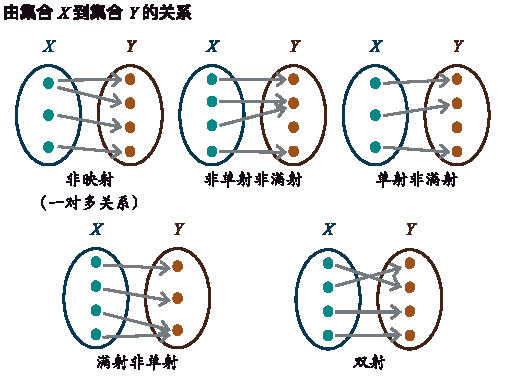
\includegraphics{../images/mapping.pdf}
    \caption{映射的不同概念示意图。}
    \label{fig:II.1.3}
\end{figure}

映射定义的第1条要求如果违反了,可通过对集合$X$的改动重新得到满足,而无需改动关系$f$本身。例如若$\mathrm{dom}f\subsetneqq X$,则令$X^\prime=\mathrm{dom}f$并改为讨论由$X^\prime$到$Y$的关系$f$,就可通过映射定义的第1条。然而映射定义的第2条如果违反了,想要重新满足就不得不对关系$f$本身进行改动。图\ref{fig:II.1.3}中的第一个例子就只是一个关系,而不是一个映射,除非我们从这一关系中拿掉一个有序对。

给定映射$f:X\rightarrow Y$,我们继续以下讨论:
\begin{itemize}
    \item 一般地,$Y$未必等于$\mathrm{ran}f$,集合$Y$称映射$f$的\emph{陪域(codomain)}。
    \item 若$E$是$X$的一个子集,若由$E$到$Y$的映射$\left.f\right|_E:E\rightarrow Y$满足$\left.f\right|_A\left(x\right)=f\left(x\right),\forall x\in E$,则称映射$\left.f\right|_E$是映射$f$在$E$上的\emph{限制(restriction)}(记法亦已表明)\footnote{通俗说$f$在$A$上的限制跟$f$是同一个映射,只不过定义在了“更小的”一个集合$A$上罢了。}。
    \item 若$\mathrm{ran}f=Y$则称映射$f$是\emph{满射(surjective mapping)}。图\ref{fig:II.1.3}中的第4和第5个例子都是满射。
    \item 若$A\subset X$,则集合$\left\{y\in Y|\forall x\left(x\in A\wedge y=f\left(x\right)\right)\right\}$称集合$A$在映射$f$下的\emph{像(image)},简记为$f\left(A\right)$。这一集合可用语言描述为:由集合$A$的所有元素在映射$f$下的值组成的集合。易证它是$Y$的子集。
    \item 若对任意$x_1,x_2\in X$,$f\left(x_1\right)=f\left(x_2\right)\Rightarrow x_1=x_2$,则称$f$是\emph{单射(injective mapping)}。可用语言描述为,“单射的输出唯一地确定其输入”。图\ref{fig:II.1.3}中的第3和第5个例子都是单射。
    \item 如果$f$既是满射又是单射,则称$f$是一个\emph{双射(bijective mapping)}。图\ref{fig:II.1.3}中的第5个例子是双射。
    \item 若另一映射$g:Y\rightarrow Z$,可与映射$f$构成从$X$到$Z$的映射$g\circ f:X\rightarrow Z$,且
          \[
              g\circ f\left(x\right)=g\left(f\left(x\right)\right),\forall x\in X
          \]
          则称$g\circ f$是$f$和$g$的\emph{复合映射(composite mapping)}。
    \item 如果$f\left(x\right)=x,\forall x\in X$,则称映射$f$是\emph{恒等映射(identity mapping)}。
    \item 如果映射$g:Y\rightarrow X$使得复合映射$g\circ f$是恒等映射,则称映射$f$是\emph{可逆的(invertible)},映射$g$是$f$的\emph{逆映射(inverse mapping)}。常将$f$的逆映射记作$f^{-1}$。
\end{itemize}

关于逆映射,有一条重要的定理——

\begin{theorem}\label{thm:II.1.2}
    双射必存在唯一逆映射。双射的逆映射也是双射。
\end{theorem}
\begin{proof}
    为了证明这一定理,我们首先证明一个引理:任一单射非满射均存在逆映射。

    设$f:X\rightarrow Y$是一个单射非满射,即$\exists y\notin\mathrm{ran}f,y\in Y$。由集合的相关定义此处必有$\left\{y|y\in\mathrm{ran}f\right\}\cup\left\{y|y\notin\mathrm{ran}f,y\in Y\right\}=Y$。

    现定义$g:Y\rightarrow X$,为使$g$为一个映射,它必须对$y\in\mathrm{ran}f$和$y\notin\mathrm{ran}f,y\in Y$均有定义。现将其定义为:
    \[
        g\left(y\right)=\left\{
        \begin{array}{ll}
            \left.x\right|_{f\left(x\right)=y}, & y\in\mathrm{ran}f           \\
            \text{任一}x\in X,                    & y\notin\mathrm{ran}f,y\in Y
        \end{array}
        \right.
    \]
    则有如下几条结论:
    \begin{enumerate}
        \item $g\left(y\right)$是映射。因为它对每一$y\in Y$均有定义且一个$y\in Y$只对应一个$x\in X$。
        \item $g$是满射。因为,仅$y\in\mathrm{ran}f$情况的定义式就已决定了$\mathrm{ran}g=X$。
        \item $g$是非单射。因为$g$是满射,再考虑$y\notin\mathrm{ran}f,y\in Y$情况的定义式,就可知$\exists x\in X$满足$x=g\left(y\right)=g\left(y^\prime\right)$,其中$y\neq y^\prime,y\in\mathrm{ran}f,y^\prime\notin\mathrm{ran}f,y^\prime\in Y$。
        \item $g$是$f$的逆映射。因为,对于任一$x\in X$均有$g\circ f\left(x\right)\equiv g\left(f\left(x\right)\right)=x$,即$g\circ f=\mathrm{id}_X$。
        \item 一般地,$g$是不唯一的。因为$y\notin\mathrm{f},y\in Y$的情况可定义$g\left(x\right)$等于任一$x\in X$,故只要集合$X$不是只有一个元素,那么$g$都不唯一。
    \end{enumerate}
    该引理证毕。

    现在正式证定理\ref{thm:II.1.2}。从上面定义的这个$g$继续,如果$g$是双射,则$g$不仅是满射,还是单射。由刚刚证完的引理,可用类似方法给$g$找一个逆映射$f^\prime:X\rightarrow Y$。而且,由于$\mathrm{ran}g\equiv X$,我们无需像定义$g$那样为$f^\prime$分出$x\notin\mathrm{ran}g,x\in X$的情况,因为不存在这种情况。故
    \[
        f^\prime\left(x\right)=\left.y\right|_{g\left(y\right)=x}
    \]
    是$g$的逆映射,且$f^\prime$是满射。而且,把$g$的定义代入上式有$f^\prime\left(x\right)=\left.y\right|_{g\left(y\right)=x}=\left.y\right|_{\left.x\right|_{f\left(x\right)=y}}=f\left(x\right)$,即$f^\prime$不是别的映射而恰为$f\left(x\right)$。即$g$的逆映射是唯一的。因$f^\prime$是满射故$f$是满射,而$f$本身就是单射,故$f$是双射。
\end{proof}

% 需要增加“族”的概念。这至少是多于2个集合的笛卡尔积的基础。
我们常把映射写成另一种形式,并给以另一个名称。具体地,当我们把由$I$到$X$的映射$x:I\rightarrow X$改称为\emph{索引族(indexed family)}时,定义域$I$就称为\emph{索引集(indexing set)},其元素$i\in I$称为\emph{索引(indexes)}。映射$x$的关于$i\in I$的值,记作$x_i$,称为该索引族的一\emph{项(term)}。映射$x$的值域,称作\emph{由$I$索引的集合(set indexed by $I$)},或笼统地称其为一个\emph{索引集(indexed set)}。我们经常不加分辨地直接把$\left\{x_i\right\}_{i\in I}$称为一个\emph{由$I$索引的族($I$-indexed family)}。可见,我们无非把映射原有概念的名称换了一套新的名称。我们经常讨论的是以集合为项的族,称为\emph{集合的索引族(indexed family of sets)}。

设$\mathcal{C}$是集合的集合。如果有$\mathcal{C}$恰好还是一个由集合$I$索引的集合,$\mathcal{C}=\left\{X_i\right\}_{i\in I}$,那么第一节介绍的$\mathcal{C}$的元素的交集和并集就相应有新的表示方式:
\[
    \bigcap_{X\in\mathcal{C}}X=\bigcap_{i\in I}X_i,\quad\bigcup_{X\in\mathcal{C}}X=\bigcup_{i\in I}X_i
\]

下面我们介绍多于两个集合的笛卡尔集的定义\footnote{第一节中引入的两个集合的笛卡尔集定义,无法推广至不可数无穷多个集合间的笛卡尔积。所以,我们在介绍了映射之后,在族的基础上可重新定义笛卡尔集。这个新的定义,在集合个数为两个的情况下,也导致一种与老定义不同的“有序对”,但是新定义和老定义得出有序对之间总是一一对应的,因此无所谓从哪种定义去理解有序对。虽然笛卡尔积的新定义既兼容两个集合间的情况(甚至把“一个集合的笛卡尔集”也定义了),又能够推广到不可数无穷个集合间的笛卡尔集,但是它却不能在一开始就采用,因为它依赖映射的定义,而映射是一种关系,关系的定义依赖有序对的定义。所以我们至少需要先以老定义获得有序对的概念,才能走到现在这一步。}

\begin{definition}[笛卡尔积]\label{def:Cartesian_product_family}
    设$\left\{S_i\right\}_{i\in I}$是由$I$索引的族,且它是集合的索引族,$\left\{s_i\right\}_{i\in I}$也是由$I$索引的族,且$s_i\in S_i,\forall i\in I$。我们称$\left\{S_i\right\}_{i\in I}$的笛卡尔积是由$\left\{S_i\right\}_{i\in I}$得出的所有族$\left\{s_i\right\}_{i\in I}$的集合,记为
    \[
        \prod_{i\in I}S_i
    \]
    若$S_i=S,\forall i\in I$,则记$\prod_{i\in I}S_i\equiv S^I$。
\end{definition}


% 这个例子的功能是让读者理解这个定义。因此需要更加step-by-step,也许要使用图形。
\begin{example}
    设$I=\left\{a,b\right\},X_a=\left\{a_\alpha,a_\beta\right\},X_b=\left\{b_\alpha,b_\beta\right\}$,则按照笛卡尔积的老定义,
    \[
        X_a\times X_b=\left\{\left(a_\alpha,b_\alpha\right),\left(a_\alpha,b_\beta\right),\left(a_\beta,b_\alpha\right),\left(a_\beta,b_\beta\right)\right\}
    \]
    其中按照有序对的老定义,$\left(x,y\right)=\left\{\left\{x\right\},\left\{x,y\right\}\right\}$。

    按照新定义\ref{def:Cartesian_product_family}的要求,我们要在$X_a$和$X_b$中各选一个元素组成由$\left\{a,b\right\}$索引的族$\left\{x_i\right\}_{i\in\left\{a,b\right\}}$。例如,令$x_a=a_\beta,x_b=b_\alpha$所形成的族$\left\{x_i\right\}_{i\in\left\{a,b\right\}}\equiv\left\{x_a,x_b\right\}=\left\{a_\beta,b_\alpha\right\}$就是其中一个符合要求的族。所有这样的族,一共有4个。因此有
    \[
        \prod_{i\in\left\{a,b\right\}}X_i=\left\{\left\{a_\alpha,b_\alpha\right\},\left\{a_\alpha,b_\beta\right\},\left\{a_\beta,b_\alpha\right\},\left\{a_\beta,b_\beta\right\}\right\}
    \]
\end{example}

% 这里要加一段设问:
% 1. 为啥要新定义?
% 2. 新定义和老定义得出的东西是不一样的。那老定义怎么办?
% 3. 为什么不一开始就按新定义?
% 4. 新老定义总是要同时写在书上。
% 5. 那在同一文本中,同一概念新老定义会冲突?
% 6. 在二元的情况下两个定义得到的东西虽然不一样,但是元素一一对应。因此不造成问题。

笛卡尔积的老定义与新定义是不冲突的。一般地,老定义下的笛卡尔积$X_a\times X_b$和新定义下的笛卡尔集$\prod_{i\in\left\{a,b\right\}}X_i$之间总可以定义一个映射$f:\prod_{i\in\left\{a,b\right\}}X_i\rightarrow X_a\times X_b,f\left(z\right)=\left(z_a,z_b\right),\forall z\equiv\left\{z_i\right\}_{i\in\left\{a,b\right\}}\in\prod_{i\in I}X_i$。记$z=\left\{z_i\right\}_{i\in\left\{a,b\right\}}$,则按定义\ref{def:Cartesian_product_family}有$z_i\in X_i,\forall i\in\left\{a,b\right\}$。可以证明$f$是双射:
\begin{proof}
    设$z=\left\{z_i\right\}_{i\in\left\{a,b\right\}},z^\prime=\left\{z^\prime_i\right\}_{i\in\left\{a,b\right\}}$且$z_a,z^\prime_a\in X_a,z_b,z^\prime_b\in X_b$。若$z\neq z^\prime$。由映射$f$的定义,$f\left(z\right)=\left(z_a,z_b\right),f\left(z^\prime\right)=\left(z^\prime_a,z^\prime_b\right)$。由集合相等的定义,$z\neq z^\prime\Rightarrow\left(z_a,z_B\right)\neq\left(z^\prime_a,z^\prime_b\right)$,即$f\left(z\right)\neq f\left(z^\prime\right)$,即$f$是非单射。

    设$\left(u,v\right)\in X_a\times X_b$\footnote{此处我们需要规定,只要集合$X$和$Y$都是非空集合,那么它们的笛卡尔集$X\times Y$也是非空集合,即必存在一$\left(x,y\right)\in X\times Y,x\in X,y\in Y$。这是集合论的\emph{选择公理(axiom of choice)}。},则以$\left\{a,b\right\}$索引的族$x\equiv\left\{x_i\right\}_{i\in\left\{a,b\right\}},x_a=u,x_b=v$满足$x_a\in X_a,x_b\in X_b$(按照笛卡尔积的老定义),按照定义\ref{def:Cartesian_product_family},有$x\in\mathrm{dom}f$。由于所选取的$X_a\times X_b$的元素$\left(u,v\right)$是任意的,上述性质对任一$X_a\times X_b$的元素都成立,故$f$是满射。

    由双射的定义,$f$是双射。
\end{proof}

% 以下需要讨论的是:
% 1. 我们从此以后就只用新定义。
% 2. 这将限制了允许我们进行笛卡尔积的情况。当我们无法为我们想要作的笛卡积设计一个映射把所要作笛卡尔积的集合转化成它们的簇,那么我们在数学上就不被允许作这种笛卡尔积,或说这样的笛卡尔积没有意义。所幸的是,这样的情况很难想象(以作者有限的知识,还未见关于这种情况不存在的证明)。
% 应该举几种例子。一是:一个一集合的集合上的笛卡尔积;几个集合之间,有重复的笛卡尔焦;X^R;……

因此,笛卡尔集的新定义\ref{def:Cartesian_product_family}在集合数为2的情况下所得到的集合,跟笛卡尔集的老定义所得到的集合,它们的元素之间是一一对应的。在此情况下老定义和新定义没有本质差别。根据笛卡尔积的新定义,“有序对”又可以定义成索引集有两个元素的族。即$\left(x,y\right)=\left\{z_i\right\}_{i\in\left\{a,b\right\}},z_a=x,z_b=y$。这时“序”的性质仍被保留,因为$\left(y,x\right)=\left\{z_i\right\}_{i\in\left\{a,b\right\}},z_a=y,z_b=x$是不同的族,故有$\left(x,y\right)\neq\left(y,x\right)$。而且,按照新定义,仅通过改变索引集元素的个数,就可方便地推广出“有序三元组”、“有序四元组”……的定义,这是比老定义更有利的地方。从今以后,笛卡尔积就不再采用老定义,而采用定义\ref{def:Cartesian_product_family}。就算若干个两两不同的集合$X,Y,\cdots$尚未成为一个索引族,由于易验任一集合的非空集合$\mathcal{C}$均可充当其自己的索引集而成为一个索引族,故由$X,Y,\cdots$组成的集合$\left\{X,Y,\cdots\right\}$总能成为一个索引族,从而它们的笛卡尔集仍可通过定义\ref{def:Cartesian_product_family}得到定义。更一般地,给定任一集合的集合$\mathcal{C}$,若$\mathcal{C}\neq\emptyset$,则它的元素的笛卡尔积可由定义\ref{def:Cartesian_product_family}记为
\[
    \prod_{X\in\mathcal{C}}X\equiv\prod_{i\in\mathcal{C}}A_i,\quad A_i=i,\forall i\in\mathcal{C}
\]

我们常讨论索引集$I$为自然数集$\mathbb{N}$的子集\footnote{本讲义默认读者常识上理解各种数集,而不再介绍它们的集合论引入。}的族,即$I\subset\mathbb{N}$。具体地,若
\[I=\left\{a,a+1,a+2,\cdots,b-2,b-1,b\right\},a,b\in\mathbb{N},a<b\]则由$I$索引的族可记为$\left\{X_i\right\}_{i=a}^b$。相应地,若该族是集合的族,则该族的交集、并集和笛卡尔积可分别记为:
\[
    \bigcap_{i=a}^b X_i,\quad\bigcup_{i=a}^b X_i,\quad\prod_{i=a}^b X_i
\]
特别地,若$X_i=X,\forall i\in I$,令$n=b-a+1$,$\left\{X_i\right\}_{i=a}^b$的笛卡尔积可记为$X^n$。例如,$\mathbb{R}^n$是所有有序实数$n$元组$\left(x_1,\cdots,x_n\right),x_1,\cdots,x_n\in\mathbb{R}$的集合。在数学中我们常常会称$\mathbb{R}^n$是“$n$维”的。因此,定义\ref{def:Cartesian_product_family}的好处是它可以支持各种无穷维空间的构造。